\documentclass[11pt,a4paper]{article}
\usepackage{amsmath}
\usepackage{amssymb}
\usepackage{graphicx}
\usepackage{verbatim}
\begin{document}
	\noindent
	Martin Lundfall, Henri Bunting, Malte Siemers, Patrik Bey
	\begin{centering}
		\section*{Exercise sheet 12 - Machine Intelligence I}
	\end{centering}
	\subsection*{12.1 - Implementation of belief propagation}
\subsubsection*{a)}
The directed acyclic graph of the network is the previously illustrated figure below.
	\begin{figure}[h]
		\caption{DAG illustrating joint probability distribution}
		\centering
		
\includegraphics[width=.5\textwidth]{graph}
	\end{figure}
\subsubsection*{b)}
First, we construct the moral graph of DAG above.
	\begin{figure}[h]
		\caption{Moral graph of the network}
		\centering
		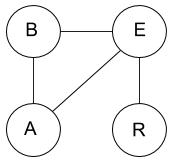
\includegraphics[width=.3\textwidth]{MORAL}
	\end{figure}
\newpage
To construct the junction tree, we compress cliques to single nodes. The node C1 is clique of $\{A, B, E\}$ in the moral graph above and the node C2 is the clique $\{E, R\}$ and the link is the separator $E$. The clique potential at C1 is the product:
\begin{equation*}
\begin{split}
P(E)P(B)P(A|B,E)=\\
P(E)P(B)\sum_{e \in E, b \in B}(P(A|e, b)\\
=0.000001\cdot 0.01\cdot\\
(0.001\cdot0.99\cdot0.99999+0.41\cdot0.99\cdot0.000001+\\
0.95\cdot0.01\cdot0.99999+0.98\cdot0.01\cdot0.000001) = 1.049^{-10}
\end{split}
\end{equation*}
The separator potential is initialized to 1. The clique potential of C2 is: $P(E)P(R|E)=P(E)=0.000001$
\begin{figure}[h]
	\caption{Junction tree of the network}
	\centering
	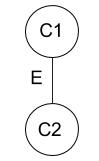
\includegraphics[width=.2\textwidth]{junction}
\end{figure}
\subsubsection*{c)}
Then we introduce the evidence. In this case, the alarm has gone off and the radio broadcasts an earthquake warning.
\end{document}
